\documentclass[1p]{elsarticle_modified}
%\bibliographystyle{elsarticle-num}

%\usepackage[colorlinks]{hyperref}
%\usepackage{abbrmath_seonhwa} %\Abb, \Ascr, \Acal ,\Abf, \Afrak
\usepackage{amsfonts}
\usepackage{amssymb}
\usepackage{amsmath}
\usepackage{amsthm}
\usepackage{scalefnt}
\usepackage{amsbsy}
\usepackage{kotex}
\usepackage{caption}
\usepackage{subfig}
\usepackage{color}
\usepackage{graphicx}
\usepackage{xcolor} %% white, black, red, green, blue, cyan, magenta, yellow
\usepackage{float}
\usepackage{setspace}
\usepackage{hyperref}

\usepackage{tikz}
\usetikzlibrary{arrows}

\usepackage{multirow}
\usepackage{array} % fixed length table
\usepackage{hhline}

%%%%%%%%%%%%%%%%%%%%%
\makeatletter
\renewcommand*\env@matrix[1][\arraystretch]{%
	\edef\arraystretch{#1}%
	\hskip -\arraycolsep
	\let\@ifnextchar\new@ifnextchar
	\array{*\c@MaxMatrixCols c}}
\makeatother %https://tex.stackexchange.com/questions/14071/how-can-i-increase-the-line-spacing-in-a-matrix
%%%%%%%%%%%%%%%

\usepackage[normalem]{ulem}

\newcommand{\msout}[1]{\ifmmode\text{\sout{\ensuremath{#1}}}\else\sout{#1}\fi}
%SOURCE: \msout is \stkout macro in https://tex.stackexchange.com/questions/20609/strikeout-in-math-mode

\newcommand{\cancel}[1]{
	\ifmmode
	{\color{red}\msout{#1}}
	\else
	{\color{red}\sout{#1}}
	\fi
}

\newcommand{\add}[1]{
	{\color{blue}\uwave{#1}}
}

\newcommand{\replace}[2]{
	\ifmmode
	{\color{red}\msout{#1}}{\color{blue}\uwave{#2}}
	\else
	{\color{red}\sout{#1}}{\color{blue}\uwave{#2}}
	\fi
}

\newcommand{\Sol}{\mathcal{S}} %segment
\newcommand{\D}{D} %diagram
\newcommand{\A}{\mathcal{A}} %arc


%%%%%%%%%%%%%%%%%%%%%%%%%%%%%5 test

\def\sl{\operatorname{\textup{SL}}(2,\Cbb)}
\def\psl{\operatorname{\textup{PSL}}(2,\Cbb)}
\def\quan{\mkern 1mu \triangleright \mkern 1mu}

\theoremstyle{definition}
\newtheorem{thm}{Theorem}[section]
\newtheorem{prop}[thm]{Proposition}
\newtheorem{lem}[thm]{Lemma}
\newtheorem{ques}[thm]{Question}
\newtheorem{cor}[thm]{Corollary}
\newtheorem{defn}[thm]{Definition}
\newtheorem{exam}[thm]{Example}
\newtheorem{rmk}[thm]{Remark}
\newtheorem{alg}[thm]{Algorithm}

\newcommand{\I}{\sqrt{-1}}
\begin{document}

%\begin{frontmatter}
%
%\title{Boundary parabolic representations of knots up to 8 crossings}
%
%%% Group authors per affiliation:
%\author{Yunhi Cho} 
%\address{Department of Mathematics, University of Seoul, Seoul, Korea}
%\ead{yhcho@uos.ac.kr}
%
%
%\author{Seonhwa Kim} %\fnref{s_kim}}
%\address{Center for Geometry and Physics, Institute for Basic Science, Pohang, 37673, Korea}
%\ead{ryeona17@ibs.re.kr}
%
%\author{Hyuk Kim}
%\address{Department of Mathematical Sciences, Seoul National University, Seoul 08826, Korea}
%\ead{hyukkim@snu.ac.kr}
%
%\author{Seokbeom Yoon}
%\address{Department of Mathematical Sciences, Seoul National University, Seoul, 08826,  Korea}
%\ead{sbyoon15@snu.ac.kr}
%
%\begin{abstract}
%We find all boundary parabolic representation of knots up to 8 crossings.
%
%\end{abstract}
%\begin{keyword}
%    \MSC[2010] 57M25 
%\end{keyword}
%
%\end{frontmatter}

%\linenumbers
%\tableofcontents
%
\newcommand\colored[1]{\textcolor{white}{\rule[-0.35ex]{0.8em}{1.4ex}}\kern-0.8em\color{red} #1}%
%\newcommand\colored[1]{\textcolor{white}{ #1}\kern-2.17ex	\textcolor{white}{ #1}\kern-1.81ex	\textcolor{white}{ #1}\kern-2.15ex\color{red}#1	}

{\Large $\underline{12n_{0165}~(K12n_{0165})}$}

\setlength{\tabcolsep}{10pt}
\renewcommand{\arraystretch}{1.6}
\vspace{1cm}\begin{tabular}{m{100pt}>{\centering\arraybackslash}m{274pt}}
\multirow{5}{120pt}{
	\centering
	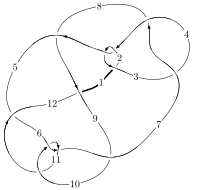
\includegraphics[width=112pt]{../../../GIT/diagram.site/Diagrams/png/2254_12n_0165.png}\\
\ \ \ A knot diagram\footnotemark}&
\allowdisplaybreaks
\textbf{Linearized knot diagam} \\
\cline{2-2}
 &
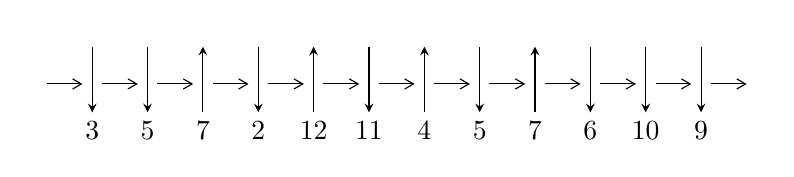
\begin{tikzpicture}[x=20pt, y=17pt]
	% nodes
	\node (C0) at (0, 0) {};
	\node (C1) at (1, 0) {};
	\node (C1U) at (1, +1) {};
	\node (C1D) at (1, -1) {3};

	\node (C2) at (2, 0) {};
	\node (C2U) at (2, +1) {};
	\node (C2D) at (2, -1) {5};

	\node (C3) at (3, 0) {};
	\node (C3U) at (3, +1) {};
	\node (C3D) at (3, -1) {7};

	\node (C4) at (4, 0) {};
	\node (C4U) at (4, +1) {};
	\node (C4D) at (4, -1) {2};

	\node (C5) at (5, 0) {};
	\node (C5U) at (5, +1) {};
	\node (C5D) at (5, -1) {12};

	\node (C6) at (6, 0) {};
	\node (C6U) at (6, +1) {};
	\node (C6D) at (6, -1) {11};

	\node (C7) at (7, 0) {};
	\node (C7U) at (7, +1) {};
	\node (C7D) at (7, -1) {4};

	\node (C8) at (8, 0) {};
	\node (C8U) at (8, +1) {};
	\node (C8D) at (8, -1) {5};

	\node (C9) at (9, 0) {};
	\node (C9U) at (9, +1) {};
	\node (C9D) at (9, -1) {7};

	\node (C10) at (10, 0) {};
	\node (C10U) at (10, +1) {};
	\node (C10D) at (10, -1) {6};

	\node (C11) at (11, 0) {};
	\node (C11U) at (11, +1) {};
	\node (C11D) at (11, -1) {10};

	\node (C12) at (12, 0) {};
	\node (C12U) at (12, +1) {};
	\node (C12D) at (12, -1) {9};
	\node (C13) at (13, 0) {};

	% arrows
	\draw[->,>={angle 60}]
	(C0) edge (C1) (C1) edge (C2) (C2) edge (C3) (C3) edge (C4) (C4) edge (C5) (C5) edge (C6) (C6) edge (C7) (C7) edge (C8) (C8) edge (C9) (C9) edge (C10) (C10) edge (C11) (C11) edge (C12) (C12) edge (C13) ;	\draw[->,>=stealth]
	(C1U) edge (C1D) (C2U) edge (C2D) (C3D) edge (C3U) (C4U) edge (C4D) (C5D) edge (C5U) (C6U) edge (C6D) (C7D) edge (C7U) (C8U) edge (C8D) (C9D) edge (C9U) (C10U) edge (C10D) (C11U) edge (C11D) (C12U) edge (C12D) ;
	\end{tikzpicture} \\
\hhline{~~} \\& 
\textbf{Solving Sequence} \\ \cline{2-2} 
 &
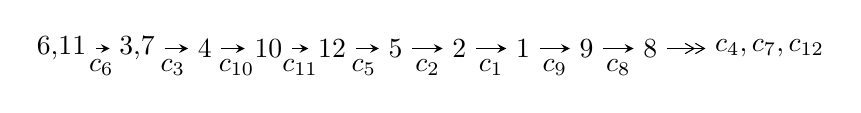
\begin{tikzpicture}[x=23pt, y=7pt]
	% node
	\node (A0) at (-1/8, 0) {6,11};
	\node (A1) at (17/16, 0) {3,7};
	\node (A2) at (17/8, 0) {4};
	\node (A3) at (25/8, 0) {10};
	\node (A4) at (33/8, 0) {12};
	\node (A5) at (41/8, 0) {5};
	\node (A6) at (49/8, 0) {2};
	\node (A7) at (57/8, 0) {1};
	\node (A8) at (65/8, 0) {9};
	\node (A9) at (73/8, 0) {8};
	\node (C1) at (1/2, -1) {$c_{6}$};
	\node (C2) at (13/8, -1) {$c_{3}$};
	\node (C3) at (21/8, -1) {$c_{10}$};
	\node (C4) at (29/8, -1) {$c_{11}$};
	\node (C5) at (37/8, -1) {$c_{5}$};
	\node (C6) at (45/8, -1) {$c_{2}$};
	\node (C7) at (53/8, -1) {$c_{1}$};
	\node (C8) at (61/8, -1) {$c_{9}$};
	\node (C9) at (69/8, -1) {$c_{8}$};
	\node (A10) at (11, 0) {$c_{4},c_{7},c_{12}$};

	% edge
	\draw[->,>=stealth]	
	(A0) edge (A1) (A1) edge (A2) (A2) edge (A3) (A3) edge (A4) (A4) edge (A5) (A5) edge (A6) (A6) edge (A7) (A7) edge (A8) (A8) edge (A9) ;
	\draw[->>,>={angle 60}]	
	(A9) edge (A10);
\end{tikzpicture} \\ 

\end{tabular} \\

\footnotetext{
The image of knot diagram is generated by the software ``\textbf{Draw programme}" developed by Andrew Bartholomew(\url{http://www.layer8.co.uk/maths/draw/index.htm\#Running-draw}), where we modified some parts for our purpose(\url{https://github.com/CATsTAILs/LinksPainter}).
}\phantom \\ \newline 
\centering \textbf{Ideals for irreducible components\footnotemark of $X_{\text{par}}$} 
 
\begin{align*}
I^u_{1}&=\langle 
- u^{41}+u^{40}+\cdots+u^2+b,\;u^{41}- u^{40}+\cdots+a+2,\;u^{42}-2 u^{41}+\cdots+2 u-1\rangle \\
I^u_{2}&=\langle 
u^6-2 u^4- u^3+u^2+b+u+1,\;u^7+u^6-2 u^5-2 u^4+u^3+u^2+a+u+1,\\
\phantom{I^u_{2}}&\phantom{= \langle  }u^9+u^8-2 u^7-3 u^6+u^5+3 u^4+2 u^3- u-1\rangle \\
\\
\end{align*}
\raggedright * 2 irreducible components of $\dim_{\mathbb{C}}=0$, with total 51 representations.\\
\footnotetext{All coefficients of polynomials are rational numbers. But the coefficients are sometimes approximated in decimal forms when there is not enough margin.}
\newpage
\renewcommand{\arraystretch}{1}
\centering \section*{I. $I^u_{1}= \langle - u^{41}+u^{40}+\cdots+u^2+b,\;u^{41}- u^{40}+\cdots+a+2,\;u^{42}-2 u^{41}+\cdots+2 u-1 \rangle$}
\flushleft \textbf{(i) Arc colorings}\\
\begin{tabular}{m{7pt} m{180pt} m{7pt} m{180pt} }
\flushright $a_{6}=$&$\begin{pmatrix}1\\0\end{pmatrix}$ \\
\flushright $a_{11}=$&$\begin{pmatrix}0\\u\end{pmatrix}$ \\
\flushright $a_{3}=$&$\begin{pmatrix}- u^{41}+u^{40}+\cdots+2 u-2\\u^{41}- u^{40}+\cdots+u^3- u^2\end{pmatrix}$ \\
\flushright $a_{7}=$&$\begin{pmatrix}1\\u^2\end{pmatrix}$ \\
\flushright $a_{4}=$&$\begin{pmatrix}- u^{40}+u^{39}+\cdots+u-1\\- u^{40}+u^{39}+\cdots-2 u^2+u\end{pmatrix}$ \\
\flushright $a_{10}=$&$\begin{pmatrix}u\\u\end{pmatrix}$ \\
\flushright $a_{12}=$&$\begin{pmatrix}- u^3\\- u^3+u\end{pmatrix}$ \\
\flushright $a_{5}=$&$\begin{pmatrix}u^6- u^4+1\\u^6-2 u^4+u^2\end{pmatrix}$ \\
\flushright $a_{2}=$&$\begin{pmatrix}u^{39}- u^{38}+\cdots+u-2\\u^{41}- u^{40}+\cdots+u^3-2 u^2\end{pmatrix}$ \\
\flushright $a_{1}=$&$\begin{pmatrix}u^{11}-2 u^9+2 u^7+u^3\\u^{13}-3 u^{11}+5 u^9-4 u^7+2 u^5+u^3- u\end{pmatrix}$ \\
\flushright $a_{9}=$&$\begin{pmatrix}u^3\\u^5- u^3+u\end{pmatrix}$ \\
\flushright $a_{8}=$&$\begin{pmatrix}u^{17}-4 u^{15}+7 u^{13}-4 u^{11}-3 u^9+6 u^7-2 u^5+u\\u^{17}-5 u^{15}+11 u^{13}-12 u^{11}+5 u^9+2 u^7-2 u^5+u\end{pmatrix}$\\&\end{tabular}
\flushleft \textbf{(ii) Obstruction class $= -1$}\\~\\
\flushleft \textbf{(iii) Cusp Shapes $= -6 u^{41}+9 u^{40}+58 u^{39}-101 u^{38}-263 u^{37}+545 u^{36}+691 u^{35}-1830 u^{34}-1021 u^{33}+4173 u^{32}+344 u^{31}-6595 u^{30}+2038 u^{29}+6914 u^{28}-5159 u^{27}-3793 u^{26}+6460 u^{25}-1008 u^{24}-4436 u^{23}+3755 u^{22}+744 u^{21}-2743 u^{20}+1497 u^{19}+47 u^{18}-1234 u^{17}+1369 u^{16}-10 u^{15}-898 u^{14}+560 u^{13}-14 u^{12}-332 u^{11}+300 u^{10}+6 u^9-87 u^8+54 u^7-69 u^6-18 u^5+67 u^4-23 u^3+7 u^2+4 u-13$}\\~\\
\newpage\renewcommand{\arraystretch}{1}
\flushleft \textbf{(iv) u-Polynomials at the component}\newline \\
\begin{tabular}{m{50pt}|m{274pt}}
Crossings & \hspace{64pt}u-Polynomials at each crossing \\
\hline $$\begin{aligned}c_{1}\end{aligned}$$&$\begin{aligned}
&u^{42}+6 u^{41}+\cdots+14 u+1
\end{aligned}$\\
\hline $$\begin{aligned}c_{2},c_{4}\end{aligned}$$&$\begin{aligned}
&u^{42}-10 u^{41}+\cdots+10 u-1
\end{aligned}$\\
\hline $$\begin{aligned}c_{3},c_{7}\end{aligned}$$&$\begin{aligned}
&u^{42}- u^{41}+\cdots+512 u+512
\end{aligned}$\\
\hline $$\begin{aligned}c_{5},c_{9}\end{aligned}$$&$\begin{aligned}
&u^{42}+6 u^{41}+\cdots-134 u-17
\end{aligned}$\\
\hline $$\begin{aligned}c_{6},c_{10}\end{aligned}$$&$\begin{aligned}
&u^{42}+2 u^{41}+\cdots-2 u-1
\end{aligned}$\\
\hline $$\begin{aligned}c_{8}\end{aligned}$$&$\begin{aligned}
&u^{42}+2 u^{41}+\cdots-2773910 u-699025
\end{aligned}$\\
\hline $$\begin{aligned}c_{11}\end{aligned}$$&$\begin{aligned}
&u^{42}+22 u^{41}+\cdots+2 u+1
\end{aligned}$\\
\hline $$\begin{aligned}c_{12}\end{aligned}$$&$\begin{aligned}
&u^{42}-2 u^{41}+\cdots+2 u+1
\end{aligned}$\\
\hline
\end{tabular}\\~\\
\newpage\renewcommand{\arraystretch}{1}
\flushleft \textbf{(v) Riley Polynomials at the component}\newline \\
\begin{tabular}{m{50pt}|m{274pt}}
Crossings & \hspace{64pt}Riley Polynomials at each crossing \\
\hline $$\begin{aligned}c_{1}\end{aligned}$$&$\begin{aligned}
&y^{42}+70 y^{41}+\cdots-202 y+1
\end{aligned}$\\
\hline $$\begin{aligned}c_{2},c_{4}\end{aligned}$$&$\begin{aligned}
&y^{42}-6 y^{41}+\cdots-14 y+1
\end{aligned}$\\
\hline $$\begin{aligned}c_{3},c_{7}\end{aligned}$$&$\begin{aligned}
&y^{42}-57 y^{41}+\cdots-4718592 y+262144
\end{aligned}$\\
\hline $$\begin{aligned}c_{5},c_{9}\end{aligned}$$&$\begin{aligned}
&y^{42}+26 y^{41}+\cdots-9490 y+289
\end{aligned}$\\
\hline $$\begin{aligned}c_{6},c_{10}\end{aligned}$$&$\begin{aligned}
&y^{42}-22 y^{41}+\cdots-2 y+1
\end{aligned}$\\
\hline $$\begin{aligned}c_{8}\end{aligned}$$&$\begin{aligned}
&y^{42}+90 y^{41}+\cdots-6627902285450 y+488635950625
\end{aligned}$\\
\hline $$\begin{aligned}c_{11}\end{aligned}$$&$\begin{aligned}
&y^{42}-2 y^{41}+\cdots-22 y+1
\end{aligned}$\\
\hline $$\begin{aligned}c_{12}\end{aligned}$$&$\begin{aligned}
&y^{42}+54 y^{41}+\cdots-2 y+1
\end{aligned}$\\
\hline
\end{tabular}\\~\\
\newpage\flushleft \textbf{(vi) Complex Volumes and Cusp Shapes}
$$\begin{array}{c|c|c}  
\text{Solutions to }I^u_{1}& \I (\text{vol} + \sqrt{-1}CS) & \text{Cusp shape}\\
 \hline 
\begin{aligned}
u &= \phantom{-}0.758535 + 0.646533 I \\
a &= \phantom{-}0.556695 + 1.198170 I \\
b &= \phantom{-}0.884685 + 1.037480 I\end{aligned}
 & \phantom{-}11.73740 + 1.53247 I & \phantom{-}0.138999 + 0.820904 I \\ \hline\begin{aligned}
u &= \phantom{-}0.758535 - 0.646533 I \\
a &= \phantom{-}0.556695 - 1.198170 I \\
b &= \phantom{-}0.884685 - 1.037480 I\end{aligned}
 & \phantom{-}11.73740 - 1.53247 I & \phantom{-}0.138999 - 0.820904 I \\ \hline\begin{aligned}
u &= -0.850409 + 0.511409 I \\
a &= \phantom{-}0.510882 + 0.992064 I \\
b &= \phantom{-}0.224665 + 0.371706 I\end{aligned}
 & \phantom{-}1.85125 + 3.14547 I & \phantom{-}0.50380 - 5.60471 I \\ \hline\begin{aligned}
u &= -0.850409 - 0.511409 I \\
a &= \phantom{-}0.510882 - 0.992064 I \\
b &= \phantom{-}0.224665 - 0.371706 I\end{aligned}
 & \phantom{-}1.85125 - 3.14547 I & \phantom{-}0.50380 + 5.60471 I \\ \hline\begin{aligned}
u &= \phantom{-}0.799944 + 0.638230 I \\
a &= -0.94309 - 1.79340 I \\
b &= -0.338330 - 1.002640 I\end{aligned}
 & \phantom{-}11.61710 - 6.48369 I & -0.21200 + 5.34025 I \\ \hline\begin{aligned}
u &= \phantom{-}0.799944 - 0.638230 I \\
a &= -0.94309 + 1.79340 I \\
b &= -0.338330 + 1.002640 I\end{aligned}
 & \phantom{-}11.61710 + 6.48369 I & -0.21200 - 5.34025 I \\ \hline\begin{aligned}
u &= \phantom{-}0.894592\phantom{ +0.000000I} \\
a &= \phantom{-}1.03594\phantom{ +0.000000I} \\
b &= \phantom{-}0.336424\phantom{ +0.000000I}\end{aligned}
 & -1.45839\phantom{ +0.000000I} & -6.12070\phantom{ +0.000000I} \\ \hline\begin{aligned}
u &= -0.674270 + 0.529870 I \\
a &= \phantom{-}0.671399 - 0.395254 I \\
b &= \phantom{-}0.627556 + 0.015747 I\end{aligned}
 & \phantom{-}2.36371 + 1.10219 I & \phantom{-}2.10234 - 2.56596 I \\ \hline\begin{aligned}
u &= -0.674270 - 0.529870 I \\
a &= \phantom{-}0.671399 + 0.395254 I \\
b &= \phantom{-}0.627556 - 0.015747 I\end{aligned}
 & \phantom{-}2.36371 - 1.10219 I & \phantom{-}2.10234 + 2.56596 I \\ \hline\begin{aligned}
u &= \phantom{-}0.229875 + 0.814047 I \\
a &= -0.318800 + 1.227780 I \\
b &= -2.11276 - 1.36196 I\end{aligned}
 & \phantom{-}8.65210 + 8.20700 I & -1.50156 - 4.22989 I\\
 \hline 
 \end{array}$$\newpage$$\begin{array}{c|c|c}  
\text{Solutions to }I^u_{1}& \I (\text{vol} + \sqrt{-1}CS) & \text{Cusp shape}\\
 \hline 
\begin{aligned}
u &= \phantom{-}0.229875 - 0.814047 I \\
a &= -0.318800 - 1.227780 I \\
b &= -2.11276 + 1.36196 I\end{aligned}
 & \phantom{-}8.65210 - 8.20700 I & -1.50156 + 4.22989 I \\ \hline\begin{aligned}
u &= \phantom{-}0.265629 + 0.793421 I \\
a &= \phantom{-}0.226149 - 0.606330 I \\
b &= \phantom{-}2.08149 + 0.30188 I\end{aligned}
 & \phantom{-}9.24719 + 0.37833 I & -0.624670 + 0.106792 I \\ \hline\begin{aligned}
u &= \phantom{-}0.265629 - 0.793421 I \\
a &= \phantom{-}0.226149 + 0.606330 I \\
b &= \phantom{-}2.08149 - 0.30188 I\end{aligned}
 & \phantom{-}9.24719 - 0.37833 I & -0.624670 - 0.106792 I \\ \hline\begin{aligned}
u &= \phantom{-}1.104060 + 0.374333 I \\
a &= \phantom{-}0.75446 + 1.54813 I \\
b &= -0.75382 + 1.34478 I\end{aligned}
 & -2.74442 - 1.12803 I & -6.06477 - 0.07417 I \\ \hline\begin{aligned}
u &= \phantom{-}1.104060 - 0.374333 I \\
a &= \phantom{-}0.75446 - 1.54813 I \\
b &= -0.75382 - 1.34478 I\end{aligned}
 & -2.74442 + 1.12803 I & -6.06477 + 0.07417 I \\ \hline\begin{aligned}
u &= -1.129850 + 0.429601 I \\
a &= \phantom{-}0.69978 - 2.03550 I \\
b &= -0.45833 - 2.41418 I\end{aligned}
 & -5.34146 + 2.73778 I & -7.76940 - 4.35221 I \\ \hline\begin{aligned}
u &= -1.129850 - 0.429601 I \\
a &= \phantom{-}0.69978 + 2.03550 I \\
b &= -0.45833 + 2.41418 I\end{aligned}
 & -5.34146 - 2.73778 I & -7.76940 + 4.35221 I \\ \hline\begin{aligned}
u &= -1.178670 + 0.271644 I \\
a &= \phantom{-}2.19851 + 0.72892 I \\
b &= \phantom{-}1.52165 - 0.58407 I\end{aligned}
 & \phantom{-}4.73543 + 2.88234 I & -5.97327 - 2.64287 I \\ \hline\begin{aligned}
u &= -1.178670 - 0.271644 I \\
a &= \phantom{-}2.19851 - 0.72892 I \\
b &= \phantom{-}1.52165 + 0.58407 I\end{aligned}
 & \phantom{-}4.73543 - 2.88234 I & -5.97327 + 2.64287 I \\ \hline\begin{aligned}
u &= -0.117108 + 0.770698 I \\
a &= \phantom{-}0.612360 - 0.464938 I \\
b &= -1.219860 + 0.084521 I\end{aligned}
 & -1.15293 - 3.18904 I & -1.05779 + 4.41031 I\\
 \hline 
 \end{array}$$\newpage$$\begin{array}{c|c|c}  
\text{Solutions to }I^u_{1}& \I (\text{vol} + \sqrt{-1}CS) & \text{Cusp shape}\\
 \hline 
\begin{aligned}
u &= -0.117108 - 0.770698 I \\
a &= \phantom{-}0.612360 + 0.464938 I \\
b &= -1.219860 - 0.084521 I\end{aligned}
 & -1.15293 + 3.18904 I & -1.05779 - 4.41031 I \\ \hline\begin{aligned}
u &= \phantom{-}1.135850 + 0.467533 I \\
a &= -0.617308 - 1.067990 I \\
b &= \phantom{-}1.12086 - 1.09303 I\end{aligned}
 & -5.06407 - 5.10089 I & -8.06417 + 3.90479 I \\ \hline\begin{aligned}
u &= \phantom{-}1.135850 - 0.467533 I \\
a &= -0.617308 + 1.067990 I \\
b &= \phantom{-}1.12086 + 1.09303 I\end{aligned}
 & -5.06407 + 5.10089 I & -8.06417 - 3.90479 I \\ \hline\begin{aligned}
u &= -1.203160 + 0.305558 I \\
a &= -2.23809 + 0.67343 I \\
b &= -0.75733 + 2.10032 I\end{aligned}
 & \phantom{-}4.19530 - 4.64476 I & -6.50760 + 1.85624 I \\ \hline\begin{aligned}
u &= -1.203160 - 0.305558 I \\
a &= -2.23809 - 0.67343 I \\
b &= -0.75733 - 2.10032 I\end{aligned}
 & \phantom{-}4.19530 + 4.64476 I & -6.50760 - 1.85624 I \\ \hline\begin{aligned}
u &= -1.132780 + 0.508544 I \\
a &= -0.90981 + 1.95883 I \\
b &= \phantom{-}0.74904 + 2.04170 I\end{aligned}
 & -1.76893 + 6.56054 I & -3.91539 - 6.62369 I \\ \hline\begin{aligned}
u &= -1.132780 - 0.508544 I \\
a &= -0.90981 - 1.95883 I \\
b &= \phantom{-}0.74904 - 2.04170 I\end{aligned}
 & -1.76893 - 6.56054 I & -3.91539 + 6.62369 I \\ \hline\begin{aligned}
u &= \phantom{-}1.192020 + 0.396256 I \\
a &= -1.338870 + 0.229283 I \\
b &= -1.18542 - 1.02127 I\end{aligned}
 & -4.97897 - 0.77808 I & -5.12685 - 0.91316 I \\ \hline\begin{aligned}
u &= \phantom{-}1.192020 - 0.396256 I \\
a &= -1.338870 - 0.229283 I \\
b &= -1.18542 + 1.02127 I\end{aligned}
 & -4.97897 + 0.77808 I & -5.12685 + 0.91316 I \\ \hline\begin{aligned}
u &= \phantom{-}0.680819 + 0.286111 I \\
a &= \phantom{-}0.32342 + 1.54495 I \\
b &= -0.624981 + 0.021795 I\end{aligned}
 & -1.21863 - 1.30834 I & -6.02556 + 4.39977 I\\
 \hline 
 \end{array}$$\newpage$$\begin{array}{c|c|c}  
\text{Solutions to }I^u_{1}& \I (\text{vol} + \sqrt{-1}CS) & \text{Cusp shape}\\
 \hline 
\begin{aligned}
u &= \phantom{-}0.680819 - 0.286111 I \\
a &= \phantom{-}0.32342 - 1.54495 I \\
b &= -0.624981 - 0.021795 I\end{aligned}
 & -1.21863 + 1.30834 I & -6.02556 - 4.39977 I \\ \hline\begin{aligned}
u &= \phantom{-}1.154970 + 0.552374 I \\
a &= \phantom{-}1.32333 - 2.31600 I \\
b &= \phantom{-}2.34332 - 0.76541 I\end{aligned}
 & \phantom{-}6.62233 - 5.39094 I & -3.64487 + 3.52784 I \\ \hline\begin{aligned}
u &= \phantom{-}1.154970 - 0.552374 I \\
a &= \phantom{-}1.32333 + 2.31600 I \\
b &= \phantom{-}2.34332 + 0.76541 I\end{aligned}
 & \phantom{-}6.62233 + 5.39094 I & -3.64487 - 3.52784 I \\ \hline\begin{aligned}
u &= -1.186050 + 0.496366 I \\
a &= -1.24916 - 1.10553 I \\
b &= -1.95101 + 0.16201 I\end{aligned}
 & -4.27225 + 7.86289 I & -4.24616 - 7.85401 I \\ \hline\begin{aligned}
u &= -1.186050 - 0.496366 I \\
a &= -1.24916 + 1.10553 I \\
b &= -1.95101 - 0.16201 I\end{aligned}
 & -4.27225 - 7.86289 I & -4.24616 + 7.85401 I \\ \hline\begin{aligned}
u &= -0.229937 + 0.670128 I \\
a &= \phantom{-}0.500950 + 0.538105 I \\
b &= \phantom{-}0.526961 - 1.227640 I\end{aligned}
 & \phantom{-}0.81664 - 2.02421 I & -0.01141 + 3.23458 I \\ \hline\begin{aligned}
u &= -0.229937 - 0.670128 I \\
a &= \phantom{-}0.500950 - 0.538105 I \\
b &= \phantom{-}0.526961 + 1.227640 I\end{aligned}
 & \phantom{-}0.81664 + 2.02421 I & -0.01141 - 3.23458 I \\ \hline\begin{aligned}
u &= \phantom{-}1.173930 + 0.546675 I \\
a &= -0.61187 + 3.18910 I \\
b &= -2.91661 + 2.11720 I\end{aligned}
 & \phantom{-}5.8554 - 13.2425 I & -4.63609 + 7.63130 I \\ \hline\begin{aligned}
u &= \phantom{-}1.173930 - 0.546675 I \\
a &= -0.61187 - 3.18910 I \\
b &= -2.91661 - 2.11720 I\end{aligned}
 & \phantom{-}5.8554 + 13.2425 I & -4.63609 - 7.63130 I \\ \hline\begin{aligned}
u &= -0.657519\phantom{ +0.000000I} \\
a &= -2.62357\phantom{ +0.000000I} \\
b &= -1.65716\phantom{ +0.000000I}\end{aligned}
 & -2.37590\phantom{ +0.000000I} & \phantom{-}1.74590\phantom{ +0.000000I}\\
 \hline 
 \end{array}$$\newpage$$\begin{array}{c|c|c}  
\text{Solutions to }I^u_{1}& \I (\text{vol} + \sqrt{-1}CS) & \text{Cusp shape}\\
 \hline 
\begin{aligned}
u &= \phantom{-}0.088074 + 0.595763 I \\
a &= -0.85711 - 1.31323 I \\
b &= -0.101404 + 0.925885 I\end{aligned}
 & -2.22400 + 0.97106 I & -5.17623 + 0.64972 I \\ \hline\begin{aligned}
u &= \phantom{-}0.088074 - 0.595763 I \\
a &= -0.85711 + 1.31323 I \\
b &= -0.101404 - 0.925885 I\end{aligned}
 & -2.22400 - 0.97106 I & -5.17623 - 0.64972 I\\
 \hline 
 \end{array}$$\newpage\newpage\renewcommand{\arraystretch}{1}
\centering \section*{II. $I^u_{2}= \langle u^6-2 u^4- u^3+u^2+b+u+1,\;u^7+u^6-2 u^5-2 u^4+u^3+u^2+a+u+1,\;u^9+u^8-2 u^7-3 u^6+u^5+3 u^4+2 u^3- u-1 \rangle$}
\flushleft \textbf{(i) Arc colorings}\\
\begin{tabular}{m{7pt} m{180pt} m{7pt} m{180pt} }
\flushright $a_{6}=$&$\begin{pmatrix}1\\0\end{pmatrix}$ \\
\flushright $a_{11}=$&$\begin{pmatrix}0\\u\end{pmatrix}$ \\
\flushright $a_{3}=$&$\begin{pmatrix}- u^7- u^6+2 u^5+2 u^4- u^3- u^2- u-1\\- u^6+2 u^4+u^3- u^2- u-1\end{pmatrix}$ \\
\flushright $a_{7}=$&$\begin{pmatrix}1\\u^2\end{pmatrix}$ \\
\flushright $a_{4}=$&$\begin{pmatrix}- u^7- u^6+2 u^5+2 u^4- u^3- u^2- u-1\\- u^6+2 u^4+u^3- u^2- u-1\end{pmatrix}$ \\
\flushright $a_{10}=$&$\begin{pmatrix}u\\u\end{pmatrix}$ \\
\flushright $a_{12}=$&$\begin{pmatrix}- u^3\\- u^3+u\end{pmatrix}$ \\
\flushright $a_{5}=$&$\begin{pmatrix}u^6- u^4+1\\u^6-2 u^4+u^2\end{pmatrix}$ \\
\flushright $a_{2}=$&$\begin{pmatrix}- u^7-2 u^6+2 u^5+3 u^4- u^3- u^2- u-2\\-2 u^6+4 u^4+u^3-2 u^2- u-1\end{pmatrix}$ \\
\flushright $a_{1}=$&$\begin{pmatrix}- u^6+u^4-1\\- u^6+2 u^4- u^2\end{pmatrix}$ \\
\flushright $a_{9}=$&$\begin{pmatrix}u^3\\u^5- u^3+u\end{pmatrix}$ \\
\flushright $a_{8}=$&$\begin{pmatrix}1\\u^2\end{pmatrix}$\\&\end{tabular}
\flushleft \textbf{(ii) Obstruction class $= 1$}\\~\\
\flushleft \textbf{(iii) Cusp Shapes $= - u^8-6 u^7+u^6+12 u^5+5 u^4-10 u^3-7 u^2-7 u-6$}\\~\\
\newpage\renewcommand{\arraystretch}{1}
\flushleft \textbf{(iv) u-Polynomials at the component}\newline \\
\begin{tabular}{m{50pt}|m{274pt}}
Crossings & \hspace{64pt}u-Polynomials at each crossing \\
\hline $$\begin{aligned}c_{1},c_{2}\end{aligned}$$&$\begin{aligned}
&(u-1)^9
\end{aligned}$\\
\hline $$\begin{aligned}c_{3},c_{7}\end{aligned}$$&$\begin{aligned}
&u^9
\end{aligned}$\\
\hline $$\begin{aligned}c_{4}\end{aligned}$$&$\begin{aligned}
&(u+1)^9
\end{aligned}$\\
\hline $$\begin{aligned}c_{5}\end{aligned}$$&$\begin{aligned}
&u^9+3 u^8+8 u^7+13 u^6+17 u^5+17 u^4+12 u^3+6 u^2+u-1
\end{aligned}$\\
\hline $$\begin{aligned}c_{6}\end{aligned}$$&$\begin{aligned}
&u^9+u^8-2 u^7-3 u^6+u^5+3 u^4+2 u^3- u-1
\end{aligned}$\\
\hline $$\begin{aligned}c_{8},c_{12}\end{aligned}$$&$\begin{aligned}
&u^9- u^8+2 u^7- u^6+3 u^5- u^4+2 u^3+u+1
\end{aligned}$\\
\hline $$\begin{aligned}c_{9}\end{aligned}$$&$\begin{aligned}
&u^9-3 u^8+8 u^7-13 u^6+17 u^5-17 u^4+12 u^3-6 u^2+u+1
\end{aligned}$\\
\hline $$\begin{aligned}c_{10}\end{aligned}$$&$\begin{aligned}
&u^9- u^8-2 u^7+3 u^6+u^5-3 u^4+2 u^3- u+1
\end{aligned}$\\
\hline $$\begin{aligned}c_{11}\end{aligned}$$&$\begin{aligned}
&u^9+5 u^8+12 u^7+15 u^6+9 u^5- u^4-4 u^3-2 u^2+u+1
\end{aligned}$\\
\hline
\end{tabular}\\~\\
\newpage\renewcommand{\arraystretch}{1}
\flushleft \textbf{(v) Riley Polynomials at the component}\newline \\
\begin{tabular}{m{50pt}|m{274pt}}
Crossings & \hspace{64pt}Riley Polynomials at each crossing \\
\hline $$\begin{aligned}c_{1},c_{2},c_{4}\end{aligned}$$&$\begin{aligned}
&(y-1)^9
\end{aligned}$\\
\hline $$\begin{aligned}c_{3},c_{7}\end{aligned}$$&$\begin{aligned}
&y^9
\end{aligned}$\\
\hline $$\begin{aligned}c_{5},c_{9}\end{aligned}$$&$\begin{aligned}
&y^9+7 y^8+20 y^7+25 y^6+5 y^5-15 y^4+22 y^2+13 y-1
\end{aligned}$\\
\hline $$\begin{aligned}c_{6},c_{10}\end{aligned}$$&$\begin{aligned}
&y^9-5 y^8+12 y^7-15 y^6+9 y^5+y^4-4 y^3+2 y^2+y-1
\end{aligned}$\\
\hline $$\begin{aligned}c_{8},c_{12}\end{aligned}$$&$\begin{aligned}
&y^9+3 y^8+8 y^7+13 y^6+17 y^5+17 y^4+12 y^3+6 y^2+y-1
\end{aligned}$\\
\hline $$\begin{aligned}c_{11}\end{aligned}$$&$\begin{aligned}
&y^9- y^8+12 y^7-7 y^6+37 y^5+y^4-10 y^2+5 y-1
\end{aligned}$\\
\hline
\end{tabular}\\~\\
\newpage\flushleft \textbf{(vi) Complex Volumes and Cusp Shapes}
$$\begin{array}{c|c|c}  
\text{Solutions to }I^u_{2}& \I (\text{vol} + \sqrt{-1}CS) & \text{Cusp shape}\\
 \hline 
\begin{aligned}
u &= -0.772920 + 0.510351 I \\
a &= -0.147032 - 1.012940 I \\
b &= -0.848670 - 0.225310 I\end{aligned}
 & \phantom{-}0.13850 + 2.09337 I & -1.56547 - 4.18932 I \\ \hline\begin{aligned}
u &= -0.772920 - 0.510351 I \\
a &= -0.147032 + 1.012940 I \\
b &= -0.848670 + 0.225310 I\end{aligned}
 & \phantom{-}0.13850 - 2.09337 I & -1.56547 + 4.18932 I \\ \hline\begin{aligned}
u &= \phantom{-}0.825933\phantom{ +0.000000I} \\
a &= -1.95176\phantom{ +0.000000I} \\
b &= -1.33142\phantom{ +0.000000I}\end{aligned}
 & -2.84338\phantom{ +0.000000I} & -16.7240\phantom{ +0.000000I} \\ \hline\begin{aligned}
u &= \phantom{-}1.173910 + 0.391555 I \\
a &= \phantom{-}0.679689 + 0.626017 I \\
b &= \phantom{-}0.25695 + 1.39155 I\end{aligned}
 & -6.01628 - 1.33617 I & -11.45029 + 1.01794 I \\ \hline\begin{aligned}
u &= \phantom{-}1.173910 - 0.391555 I \\
a &= \phantom{-}0.679689 - 0.626017 I \\
b &= \phantom{-}0.25695 - 1.39155 I\end{aligned}
 & -6.01628 + 1.33617 I & -11.45029 - 1.01794 I \\ \hline\begin{aligned}
u &= -0.141484 + 0.739668 I \\
a &= -0.541407 + 0.753907 I \\
b &= \phantom{-}0.443165 - 0.284059 I\end{aligned}
 & -2.26187 - 2.45442 I & -5.68179 + 2.62939 I \\ \hline\begin{aligned}
u &= -0.141484 - 0.739668 I \\
a &= -0.541407 - 0.753907 I \\
b &= \phantom{-}0.443165 + 0.284059 I\end{aligned}
 & -2.26187 + 2.45442 I & -5.68179 - 2.62939 I \\ \hline\begin{aligned}
u &= -1.172470 + 0.500383 I \\
a &= \phantom{-}0.484630 + 0.655708 I \\
b &= \phantom{-}1.314260 + 0.168567 I\end{aligned}
 & -5.24306 + 7.08493 I & -8.94033 - 5.11095 I \\ \hline\begin{aligned}
u &= -1.172470 - 0.500383 I \\
a &= \phantom{-}0.484630 - 0.655708 I \\
b &= \phantom{-}1.314260 - 0.168567 I\end{aligned}
 & -5.24306 - 7.08493 I & -8.94033 + 5.11095 I\\
 \hline 
 \end{array}$$\newpage
\newpage\renewcommand{\arraystretch}{1}
\centering \section*{ III. u-Polynomials}
\begin{tabular}{m{50pt}|m{274pt}}
Crossings & \hspace{64pt}u-Polynomials at each crossing \\
\hline $$\begin{aligned}c_{1}\end{aligned}$$&$\begin{aligned}
&((u-1)^9)(u^{42}+6 u^{41}+\cdots+14 u+1)
\end{aligned}$\\
\hline $$\begin{aligned}c_{2}\end{aligned}$$&$\begin{aligned}
&((u-1)^9)(u^{42}-10 u^{41}+\cdots+10 u-1)
\end{aligned}$\\
\hline $$\begin{aligned}c_{3},c_{7}\end{aligned}$$&$\begin{aligned}
&u^9(u^{42}- u^{41}+\cdots+512 u+512)
\end{aligned}$\\
\hline $$\begin{aligned}c_{4}\end{aligned}$$&$\begin{aligned}
&((u+1)^9)(u^{42}-10 u^{41}+\cdots+10 u-1)
\end{aligned}$\\
\hline $$\begin{aligned}c_{5}\end{aligned}$$&$\begin{aligned}
&(u^9+3 u^8+8 u^7+13 u^6+17 u^5+17 u^4+12 u^3+6 u^2+u-1)\\
&\cdot(u^{42}+6 u^{41}+\cdots-134 u-17)
\end{aligned}$\\
\hline $$\begin{aligned}c_{6}\end{aligned}$$&$\begin{aligned}
&(u^9+u^8+\cdots- u-1)(u^{42}+2 u^{41}+\cdots-2 u-1)
\end{aligned}$\\
\hline $$\begin{aligned}c_{8}\end{aligned}$$&$\begin{aligned}
&(u^9- u^8+2 u^7- u^6+3 u^5- u^4+2 u^3+u+1)\\
&\cdot(u^{42}+2 u^{41}+\cdots-2773910 u-699025)
\end{aligned}$\\
\hline $$\begin{aligned}c_{9}\end{aligned}$$&$\begin{aligned}
&(u^9-3 u^8+8 u^7-13 u^6+17 u^5-17 u^4+12 u^3-6 u^2+u+1)\\
&\cdot(u^{42}+6 u^{41}+\cdots-134 u-17)
\end{aligned}$\\
\hline $$\begin{aligned}c_{10}\end{aligned}$$&$\begin{aligned}
&(u^9- u^8+\cdots- u+1)(u^{42}+2 u^{41}+\cdots-2 u-1)
\end{aligned}$\\
\hline $$\begin{aligned}c_{11}\end{aligned}$$&$\begin{aligned}
&(u^9+5 u^8+12 u^7+15 u^6+9 u^5- u^4-4 u^3-2 u^2+u+1)\\
&\cdot(u^{42}+22 u^{41}+\cdots+2 u+1)
\end{aligned}$\\
\hline $$\begin{aligned}c_{12}\end{aligned}$$&$\begin{aligned}
&(u^9- u^8+\cdots+u+1)(u^{42}-2 u^{41}+\cdots+2 u+1)
\end{aligned}$\\
\hline
\end{tabular}\newpage\renewcommand{\arraystretch}{1}
\centering \section*{ IV. Riley Polynomials}
\begin{tabular}{m{50pt}|m{274pt}}
Crossings & \hspace{64pt}Riley Polynomials at each crossing \\
\hline $$\begin{aligned}c_{1}\end{aligned}$$&$\begin{aligned}
&((y-1)^9)(y^{42}+70 y^{41}+\cdots-202 y+1)
\end{aligned}$\\
\hline $$\begin{aligned}c_{2},c_{4}\end{aligned}$$&$\begin{aligned}
&((y-1)^9)(y^{42}-6 y^{41}+\cdots-14 y+1)
\end{aligned}$\\
\hline $$\begin{aligned}c_{3},c_{7}\end{aligned}$$&$\begin{aligned}
&y^9(y^{42}-57 y^{41}+\cdots-4718592 y+262144)
\end{aligned}$\\
\hline $$\begin{aligned}c_{5},c_{9}\end{aligned}$$&$\begin{aligned}
&(y^9+7 y^8+20 y^7+25 y^6+5 y^5-15 y^4+22 y^2+13 y-1)\\
&\cdot(y^{42}+26 y^{41}+\cdots-9490 y+289)
\end{aligned}$\\
\hline $$\begin{aligned}c_{6},c_{10}\end{aligned}$$&$\begin{aligned}
&(y^9-5 y^8+12 y^7-15 y^6+9 y^5+y^4-4 y^3+2 y^2+y-1)\\
&\cdot(y^{42}-22 y^{41}+\cdots-2 y+1)
\end{aligned}$\\
\hline $$\begin{aligned}c_{8}\end{aligned}$$&$\begin{aligned}
&(y^9+3 y^8+8 y^7+13 y^6+17 y^5+17 y^4+12 y^3+6 y^2+y-1)\\
&\cdot(y^{42}+90 y^{41}+\cdots-6627902285450 y+488635950625)
\end{aligned}$\\
\hline $$\begin{aligned}c_{11}\end{aligned}$$&$\begin{aligned}
&(y^9- y^8+12 y^7-7 y^6+37 y^5+y^4-10 y^2+5 y-1)\\
&\cdot(y^{42}-2 y^{41}+\cdots-22 y+1)
\end{aligned}$\\
\hline $$\begin{aligned}c_{12}\end{aligned}$$&$\begin{aligned}
&(y^9+3 y^8+8 y^7+13 y^6+17 y^5+17 y^4+12 y^3+6 y^2+y-1)\\
&\cdot(y^{42}+54 y^{41}+\cdots-2 y+1)
\end{aligned}$\\
\hline
\end{tabular}
\vskip 2pc
\end{document}